\section{Implementation}

\subsection{Introduction of the systems used}

For the first implementation of basic filtering operations, the evaluation board \textit{Nucleo-H743ZI} of STMicroelectronics
is used. The breakout board \textit{PmodI2S Stereo IN/OUT} is used in order to sample audio data from a 3,5\,mm jack input.

The choice for the \ac{IDE} fell on the
\newline \textit{STM32CubeIDE} as it provides an easy to use installation and
development process.

Digital filters need filter coefficients. For the first approach these
coefficients were computed beforehand and then stored in the memory of the microcontroller. For these computations,
own Python scripts were developed.

In order to design the \ac{PCB}, the \ac{EDA}-software \textit{KiCAD} was used.

\subsection{Development of the PCB}

In order to get a handy pedal, the whole hardware should be integrated into one single \ac{PCB}.
The dimensions of this should not exceed the standard size of effect pedals. As a reference the
\textit{Boss DS-1} distortion pedal were used to derive a reasonable size for the \ac{PCB}. The dimensions of the
distortion pedal are 73 x 129\,mm, which should not be exceeded. The final \ac{PCB} now has dimensions of
56,39 x 84,33\,mm.

Furthermore, there should be enough inputs, to provide the ability to extend the functionality of this board.
The idea is, to develop a platform, where any effect can be implemented. In order to fulfill this, three analog and
four digital inputs are connected to solderpads for later use. Additionally, an \ac{I2C} connector is also
provided, if for example a little display should be used.

The main components that were chosen are:

\begin{itemize}
    \item STM32H725 microcontroller
    \item CS5343-CZZ Audio \ac{DAC}
    \item CS4344-CZZR Audio \ac{ADC}
\end{itemize}

The reason for the choice of these components is that these are also present on the Nucleo- and the
breakout-board, except for the microcontroller. Therefore the smallest package with 68 pins were chosen.

A blockdiagram of the \ac{PCB} is shown in the following figure.

\begin{figure}[!h]
    \centering
    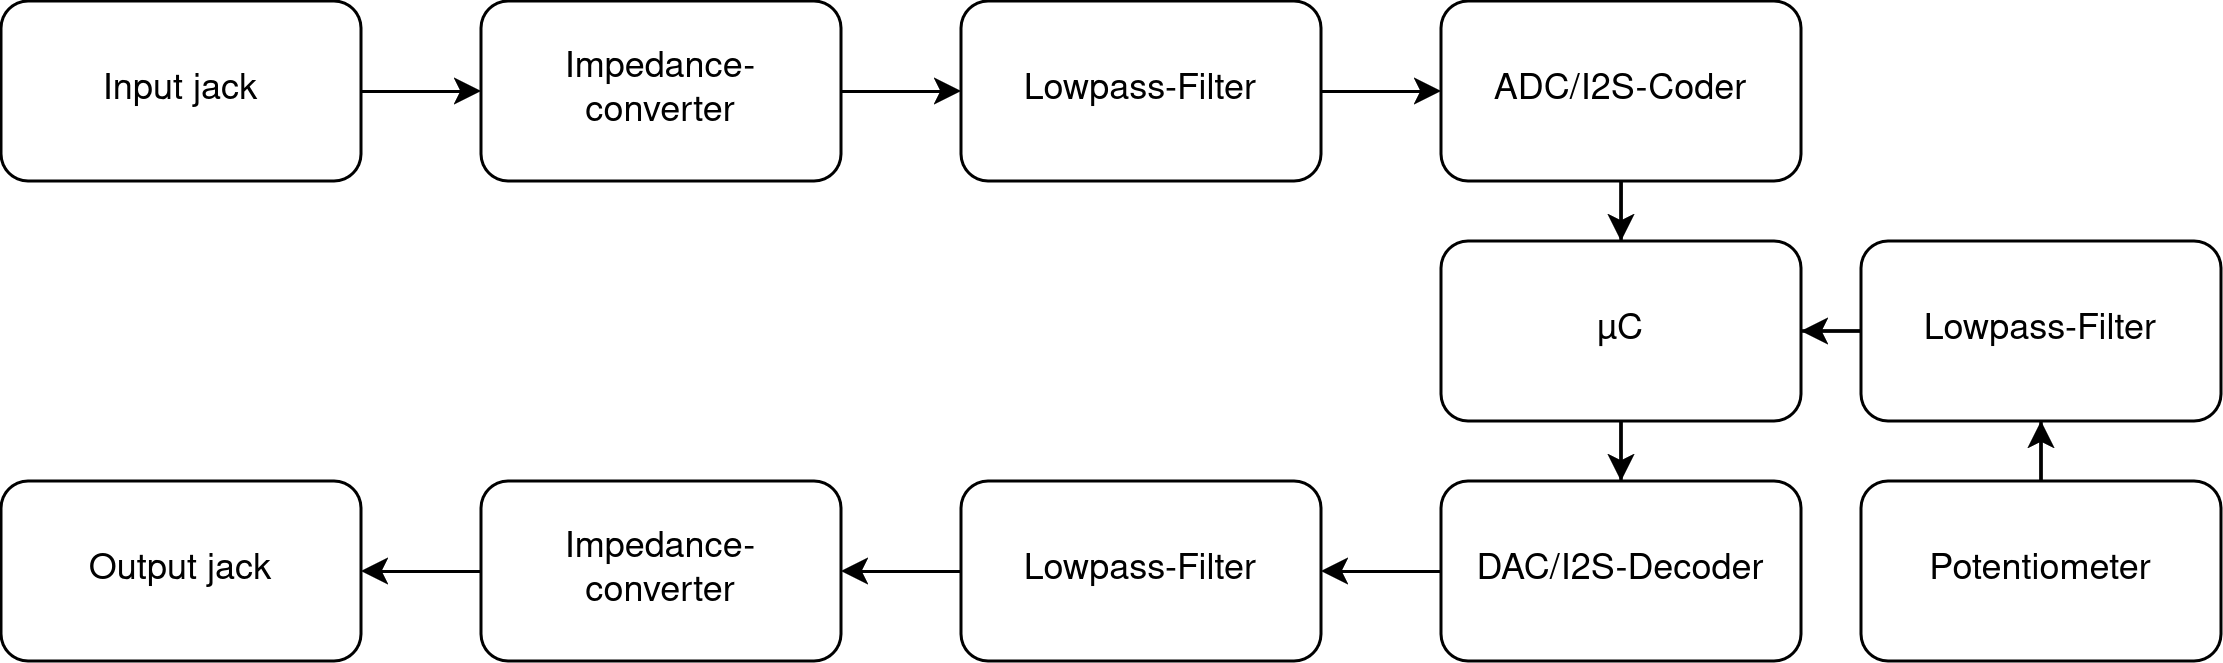
\includegraphics[width=\textwidth]{img/blockdiagram.png}
    \caption{Blockdiagram of the PCB}
    \label{fig:blockdiagram}
\end{figure}

\subsection{Implementation of the filters}

\subsubsection{Implementation using \ac{FIR}-filters}

For the first tries, \ac{FIR}-filters were used, because they always guarantee stability \cite{meyer_signalverarbeitung}.
The first prototype of the coefficients combines a set of 32 coefficient sets, which were calculated beforehand,
using the python scripts, with the following parameters:

\begin{table}[!h]
    \centering
    \caption{Parameters for \ac{FIR}-filterdesign}
    \label{table:fir-filterdesign}
    \begin{tabular}{c | c }
        quality factor & number of coefficients\\
        \hline
        5 & 130
    \end{tabular}
\end{table}

\autoref{fig:fir-sim-hamming} shows a \ac{FIR}-model of the analog reference at the lowest and (460\,Hz) and the highest
frequency (2242\,Hz). These filters are generated by using the window-method with the Hamming-window.
Also the Blackman- and the Bartlett window are tested. These simulation results are found in
\autoref{fig:fir-sim-blackman} and \autoref{fig:fir-sim-bartlett}.

\begin{figure}[!h]
    \centering
    \begin{subfigure}[c]{0.49\textwidth}
        \centering
        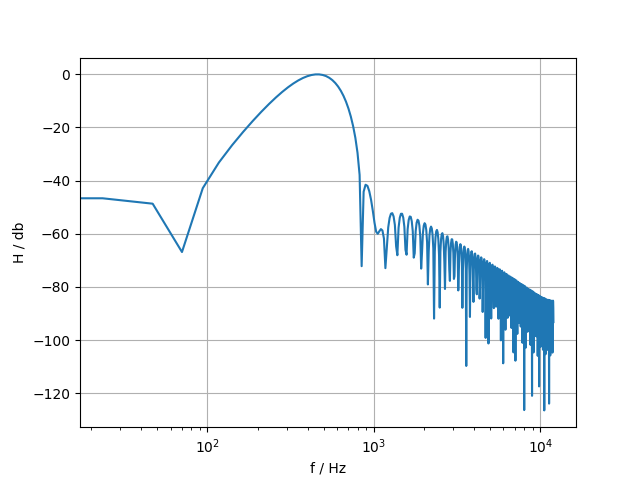
\includegraphics[width=\textwidth]{img/fir_bandpass460_hamming.png}
    \end{subfigure}
    \begin{subfigure}[c]{0.49\textwidth}
        \centering
        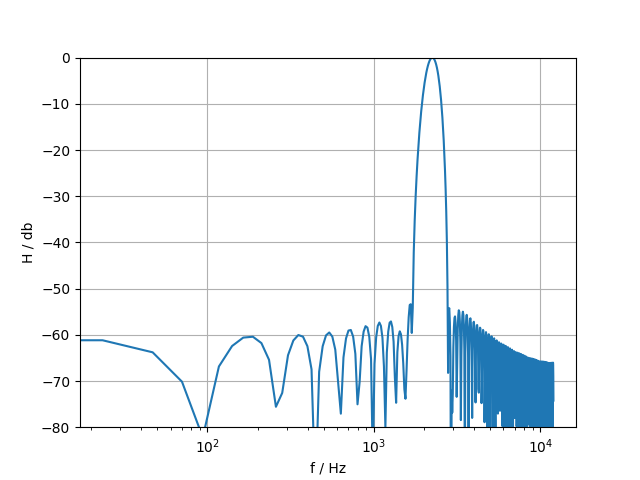
\includegraphics[width=\textwidth]{img/fir_bandpass2242_hamming.png}
    \end{subfigure}
    \caption{Simulation of the \ac{FIR}-model frequency response at 460\,Hz and 2242\,Hz using the Hamming-window}
    \label{fig:fir-sim-hamming}
\end{figure}

\begin{figure}[!h]
    \centering
    \begin{subfigure}[c]{0.49\textwidth}
        \centering
        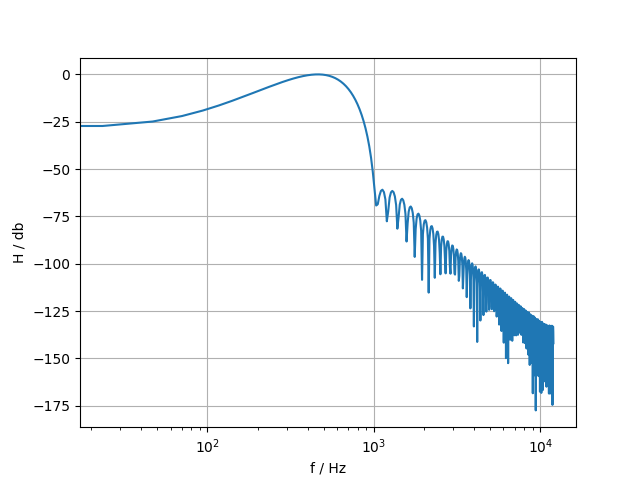
\includegraphics[width=\textwidth]{img/fir_bandpass460_blackman.png}
    \end{subfigure}
    \begin{subfigure}[c]{0.49\textwidth}
        \centering
        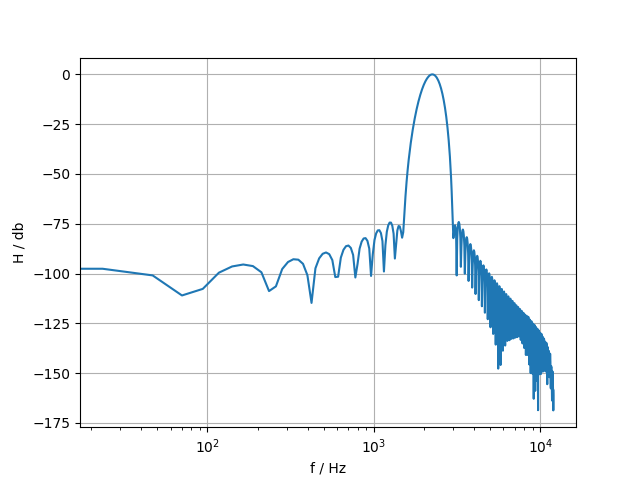
\includegraphics[width=\textwidth]{img/fir_bandpass2242_blackman.png}
    \end{subfigure}
    \caption{Simulation of the \ac{FIR}-model frequency response at 460\,Hz and 2242\,Hz using the Blackman-window}
    \label{fig:fir-sim-blackman}
\end{figure}

\begin{figure}[!h]
    \centering
    \begin{subfigure}[c]{0.49\textwidth}
        \centering
        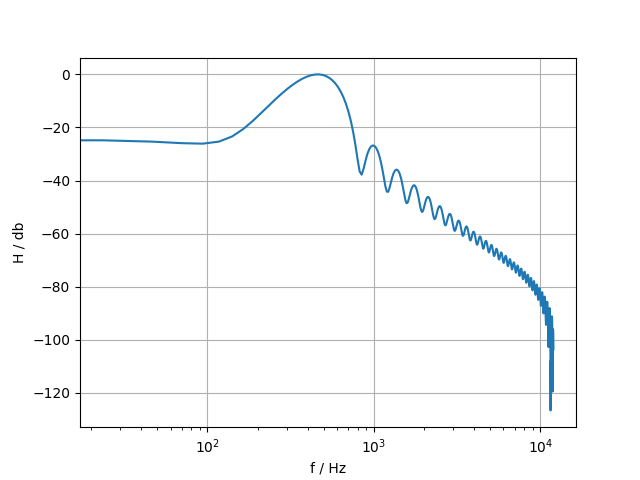
\includegraphics[width=\textwidth]{img/fir_bandpass460_bartlett.png}
    \end{subfigure}
    \begin{subfigure}[c]{0.49\textwidth}
        \centering
        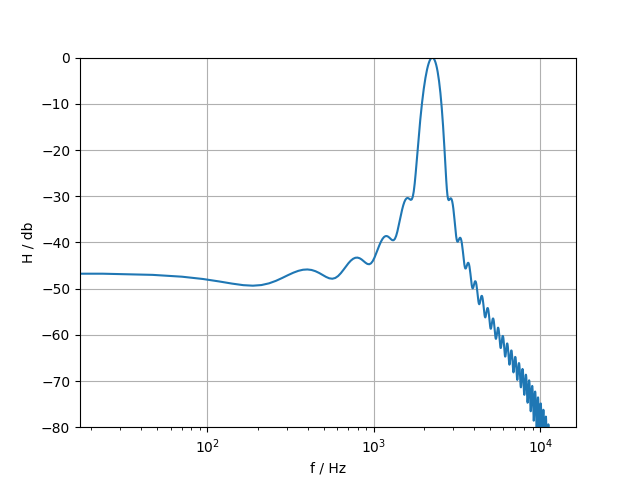
\includegraphics[width=\textwidth]{img/fir_bandpass2242_bartlett.png}
    \end{subfigure}
    \caption{Simulation of the \ac{FIR}-model frequency response at 460\,Hz and 2242\,Hz using the Bartlett-window}
    \label{fig:fir-sim-bartlett}
\end{figure}

%\cleardoublepage

It can be clearly observed, that the shape of the filters are not close to the analog reference.
The filter edges, especially near DC, are not as sharp as the actual measured reference filter.

The flowchart of the software using the \ac{FIR}-filters is shown in \autoref{fig:fir-flowchart}.

\begin{figure}[!h]
    \centering
    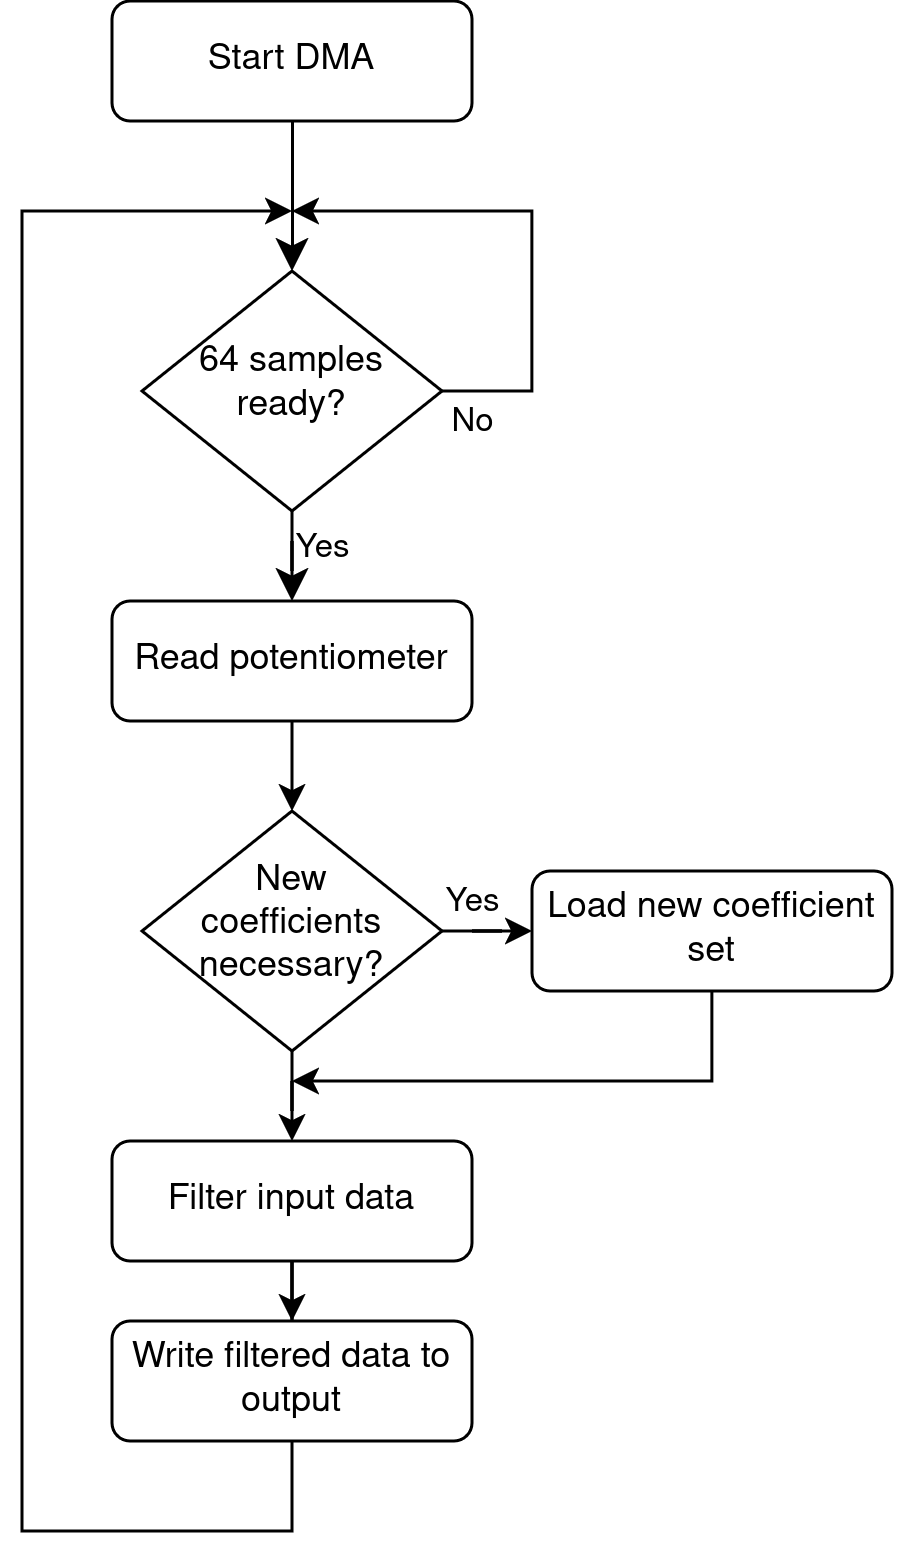
\includegraphics[width=6cm]{img/FIR_flowchart.png}
    \caption{Flowchart of the signal processing using the \ac{FIR}-filter}
    \label{fig:fir-flowchart}
\end{figure}

\cleardoublepage

\subsubsection{Implementation using biquad-filters}

The second approach to model the filter is by using a biquad-filter \cite{arm_dsp}.
As already mentioned, the filter coefficients are being calculated at runtime.

Therefore following equations are used \cite{cookbook_audio}:

\begin{align}
    \omega_0 = 2 \pi \cdot \frac{f_c}{f_s}\\
    \alpha = \frac{\sin{\omega_0}}{2 \cdot Q}\\
    b_0 = \alpha\\
    b_1 = 0\\
    b_2 = -\alpha\\
    a_0 = 1 + \alpha\\
    a_1 = -2 \cdot \cos(\omega_0)\\
    a_2 = 1 - \alpha
\end{align}

where $f_c$ is the wanted center frequency, $f_s$ the sampling frequency and $Q$ the quality factor.

Designing a bandpass-filter in biquad-structure results in the frequency responses shown in \autoref{fig:iir-biquad-sim}.

\begin{figure}[!h]
    \centering
    \begin{subfigure}[c]{0.49\textwidth}
        \centering
        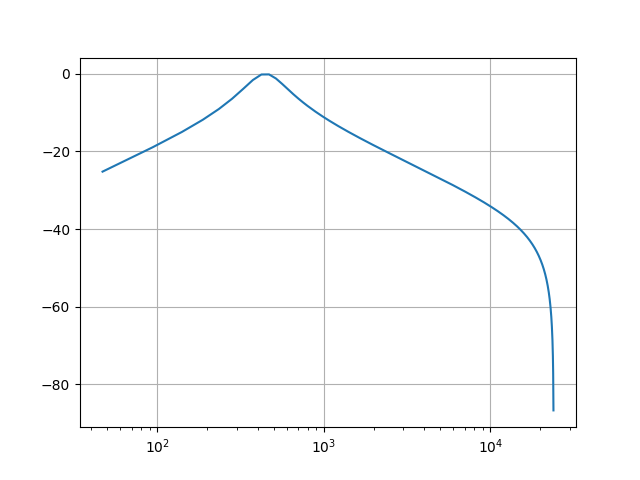
\includegraphics[width=\textwidth]{img/iir_bandpass460.png}
    \end{subfigure}
    \begin{subfigure}[c]{0.49\textwidth}
        \centering
        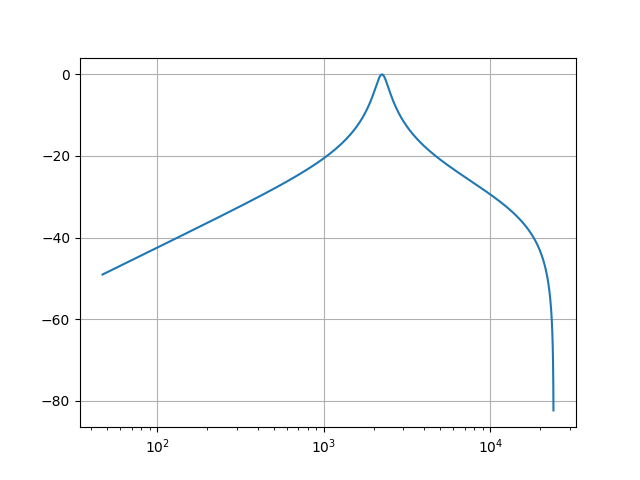
\includegraphics[width=\textwidth]{img/iir_bandpass2242.png}
    \end{subfigure}
    \caption{Simulation of the \ac{IIR}-model frequency response at 460\,Hz and 2300\,Hz}
    \label{fig:iir-biquad-sim}
\end{figure}

It shows that the edges of a biquad-filter with five coefficients are sharper than a \ac{FIR}-filter
with 130 coefficients. Also it can be seen that there is a lower attenuation in the stopband in comparison
to the \ac{FIR}-filter implementation.

In general, the overall shape is closer to the analog reference in comparison to
the non-recursive filters.

The following flowchart shows the signal processing by using the Biquad-filters.

\begin{figure}[!h]
    \centering
    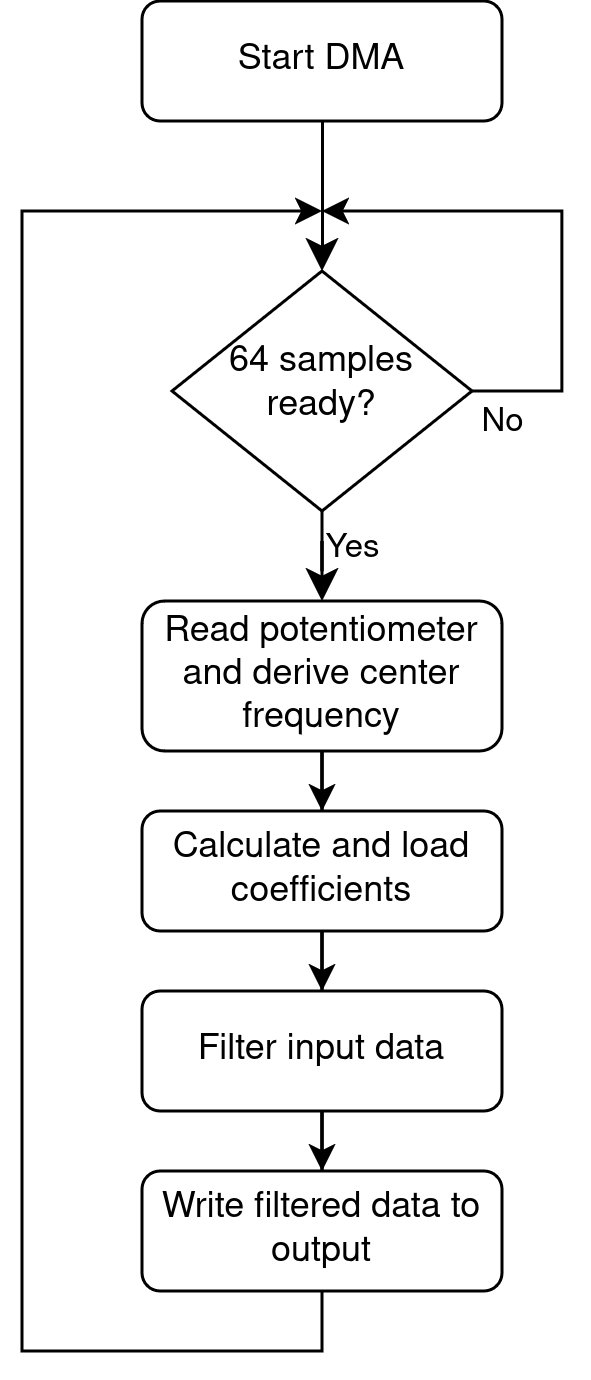
\includegraphics[width=4.5cm]{img/IIR_flowchart.png}
    \caption{Flowchart of the signal processing using the Biquad-filter}
    \label{fig:iir-flowchart}
\end{figure}

\cleardoublepage
